\documentclass[10pt]{beamer}

\usetheme{metropolis}

\usepackage{fontspec}
\setsansfont[BoldFont={Fira Sans SemiBold}]{Fira Sans Book}
\setsansfont{Fira Sans}
\setmonofont{Fira Mono}

\usepackage{appendixnumberbeamer}

\usepackage{booktabs}

\title{EL 1207 - Rangkaian Listrik 2}

\subtitle{Frekuensi Kompleks, Respon Frekuensi, dan Resonansi}

\date{\today}

\author{Mifta Nur Farid, S.T., M.T.}

\institute{Teknik Elektro - Institut Teknologi Kalimantan \\ Karang Joang, Balikpapan}

\titlegraphic{\hfill
\includegraphics[height=1.5cm]{OK-LOGO-ITK.jpg}}

\begin{document}

\maketitle

\section{Frekuensi Kompleks}

\begin{frame}{Frekuensi Kompleks}
    \begin{itemize}
        \item Frekuensi kompleks = Fungsi Sinusoidal + Konstanta Peredam
        \item Fungsi Sinusoidal $$ V_m \cos(\omega t + \theta) $$
        \item Konstanta Peredam $$ e^{\sigma t} $$ dimana $\sigma$ adalah faktor peredam atau frekuensi Neper dengan satuan $Np/s$
        \item Fungsi Sinusoidal dengan berbagai konstanta peredam dapat digambarkan dalam bentuk kurva
    \end{itemize}    
\end{frame}

\begin{frame}{Frekuensi Kompleks}
    \begin{itemize}
        \item Nilai $ \sigma = 0 $ dan $ \omega = 0 $ maka $ v(t) = V_m $
    \end{itemize}
    
    \begin{figure}
        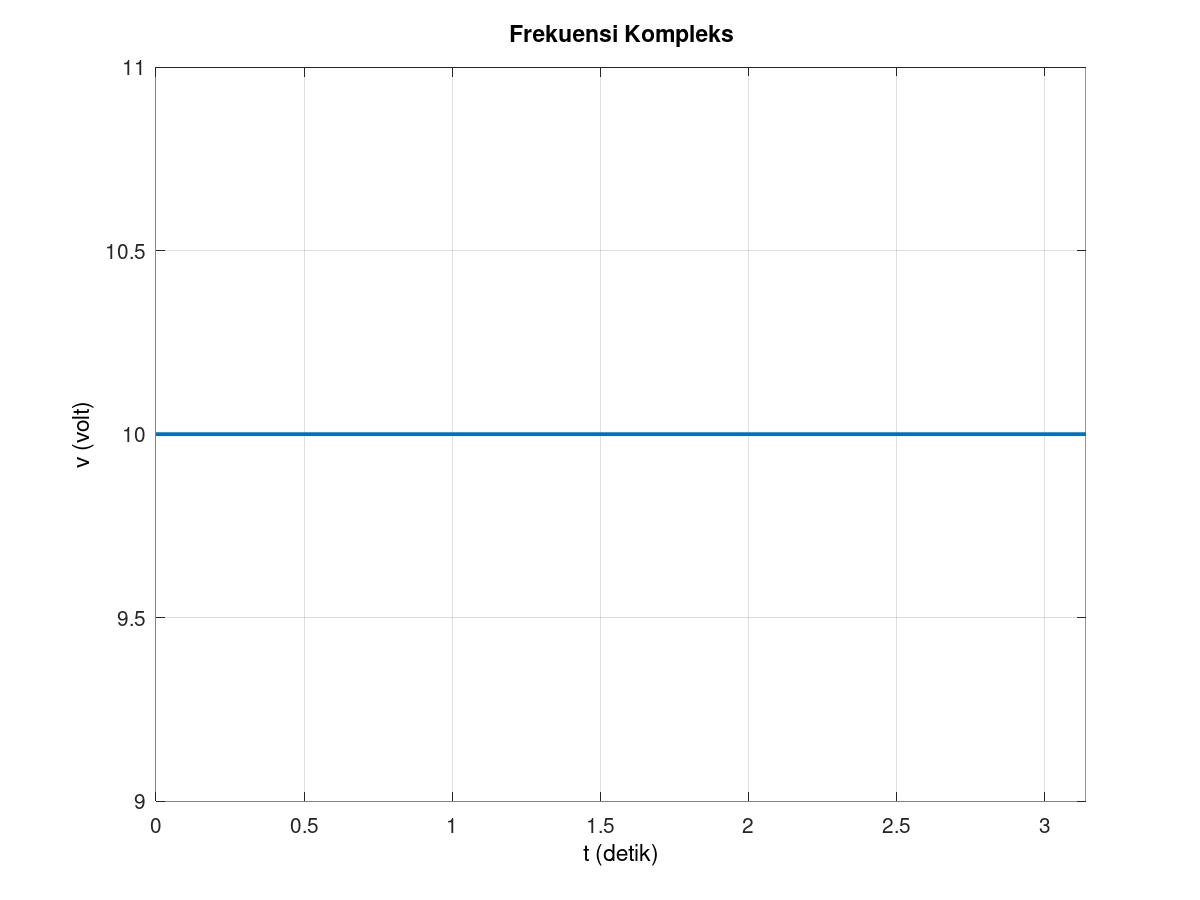
\includegraphics[width=0.8\linewidth]{gambar1.jpg}
    \end{figure}
\end{frame}

\begin{frame}{Frekuensi Kompleks}
    \begin{itemize}
        \item Nilai $ \sigma = 0 $ maka $ v(t) = V_m \cos(\omega t + \theta) $
    \end{itemize}
    
    \begin{figure}
        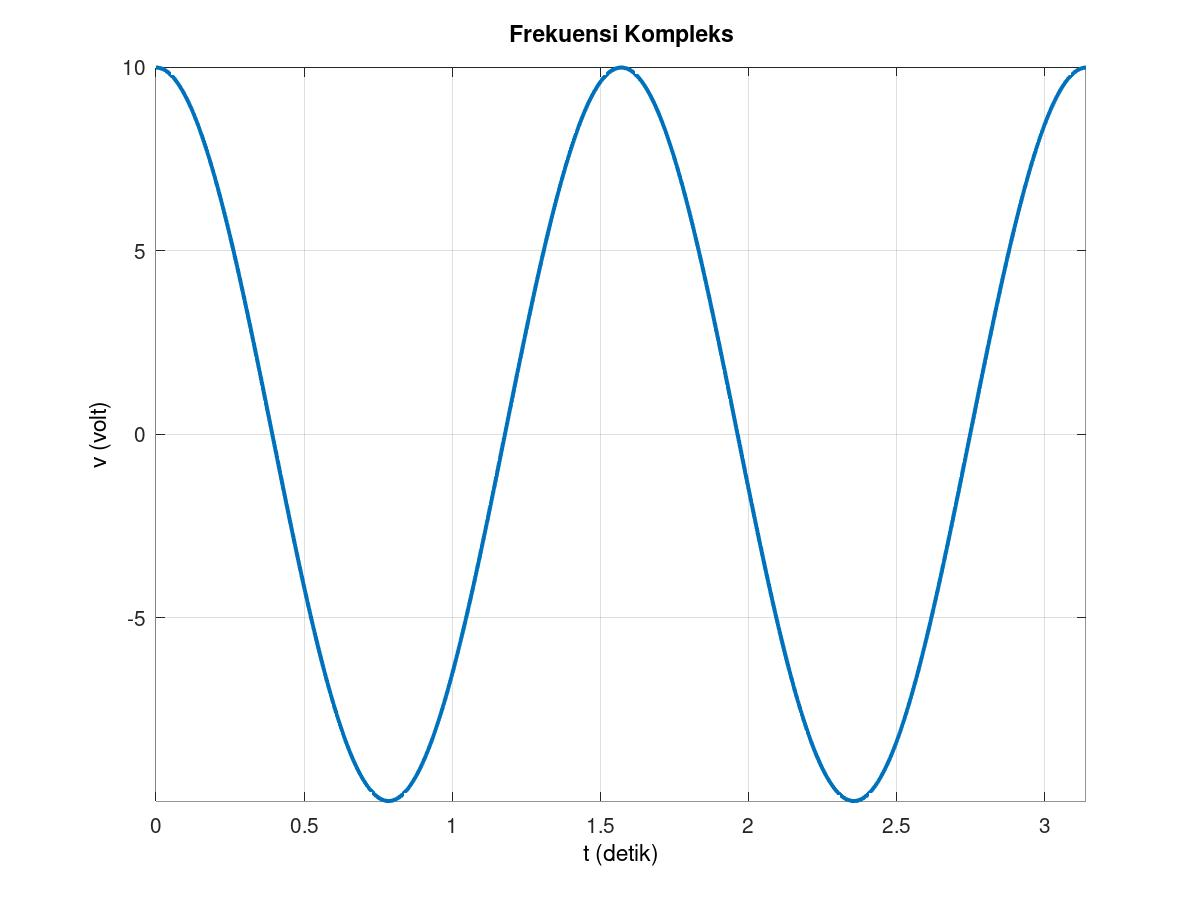
\includegraphics[width=0.8\linewidth]{gambar2.jpg}
    \end{figure}
\end{frame}

\begin{frame}{Frekuensi Kompleks}
    \begin{itemize}
        \item Nilai $ \sigma > 0 $ dan $ \omega = 0 $ maka $ v(t) = V_m e^{\sigma t} $
    \end{itemize}
    
    \begin{figure}
        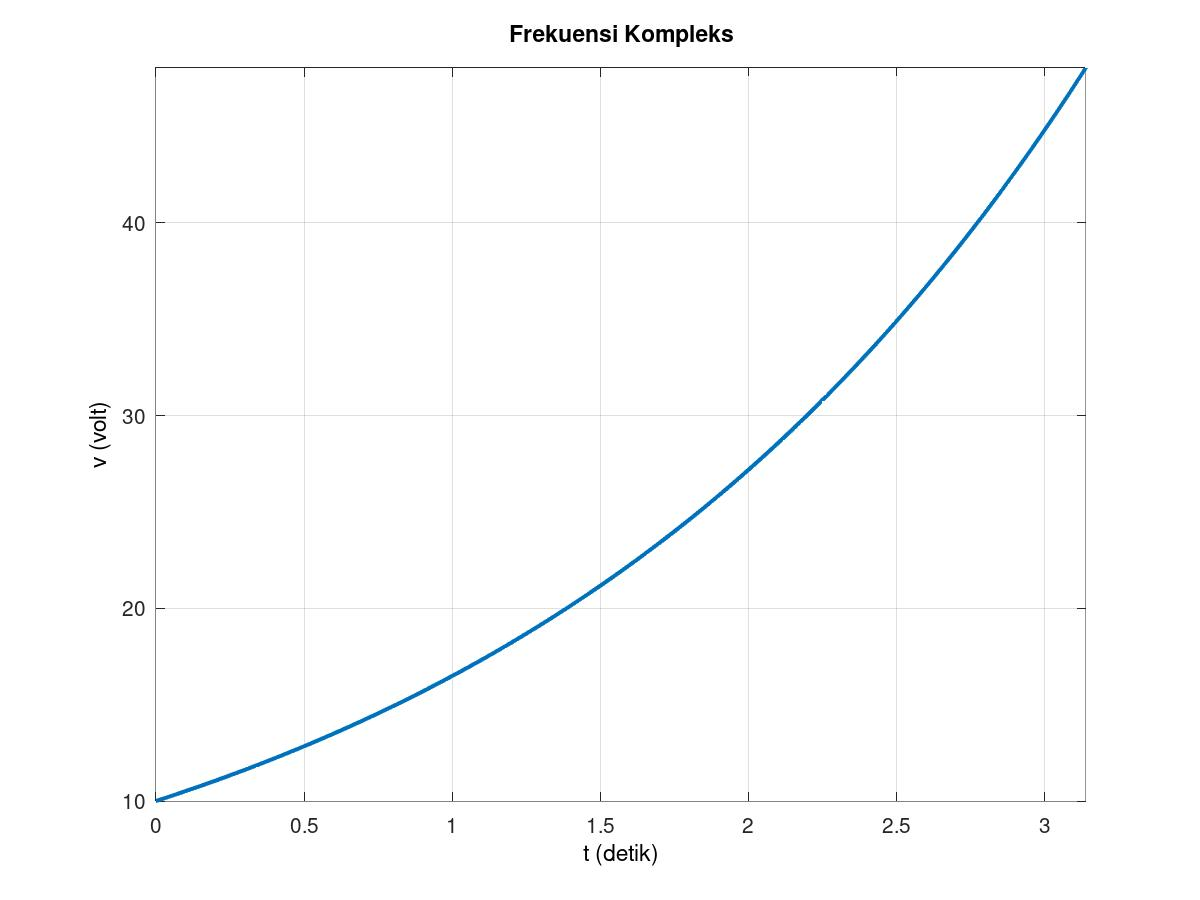
\includegraphics[width=0.8\linewidth]{gambar3.jpg}
    \end{figure}
\end{frame}

\begin{frame}{Frekuensi Kompleks}
    \begin{itemize}
        \item Nilai $\sigma < 0$ dan $\omega - 0$ maka $v(t) = V_m e^{\sigma t}$
    \end{itemize}
    \begin{figure}
        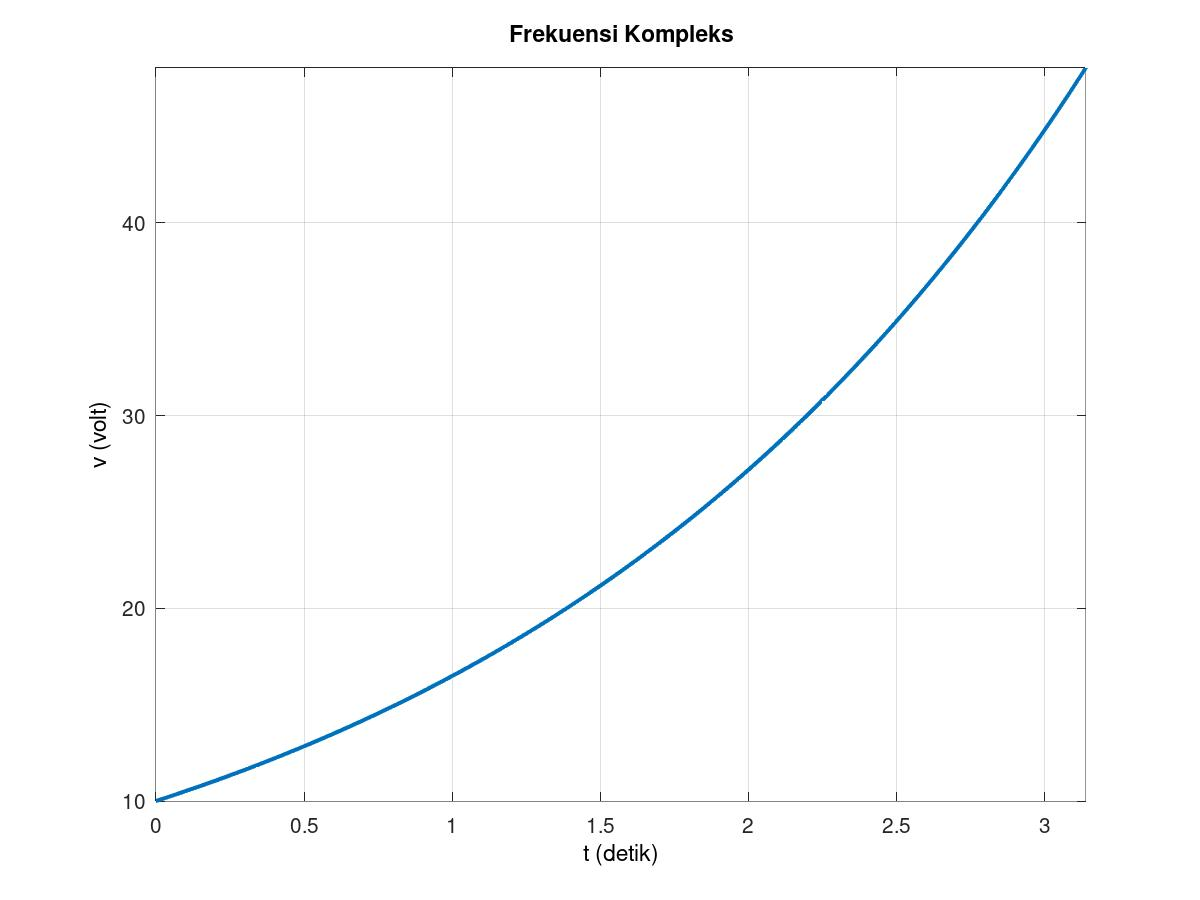
\includegraphics[width=0.8\linewidth]{gambar4.jpg}
    \end{figure}
\end{frame}

\begin{frame}{Frekuensi Kompleks}
    \begin{itemize}
        \item Nilai $\sigma > 0$ maka $v(t) = V_m e^{\sigma t} \cos(\omega t + \theta) $
    \end{itemize}
    \begin{figure}
        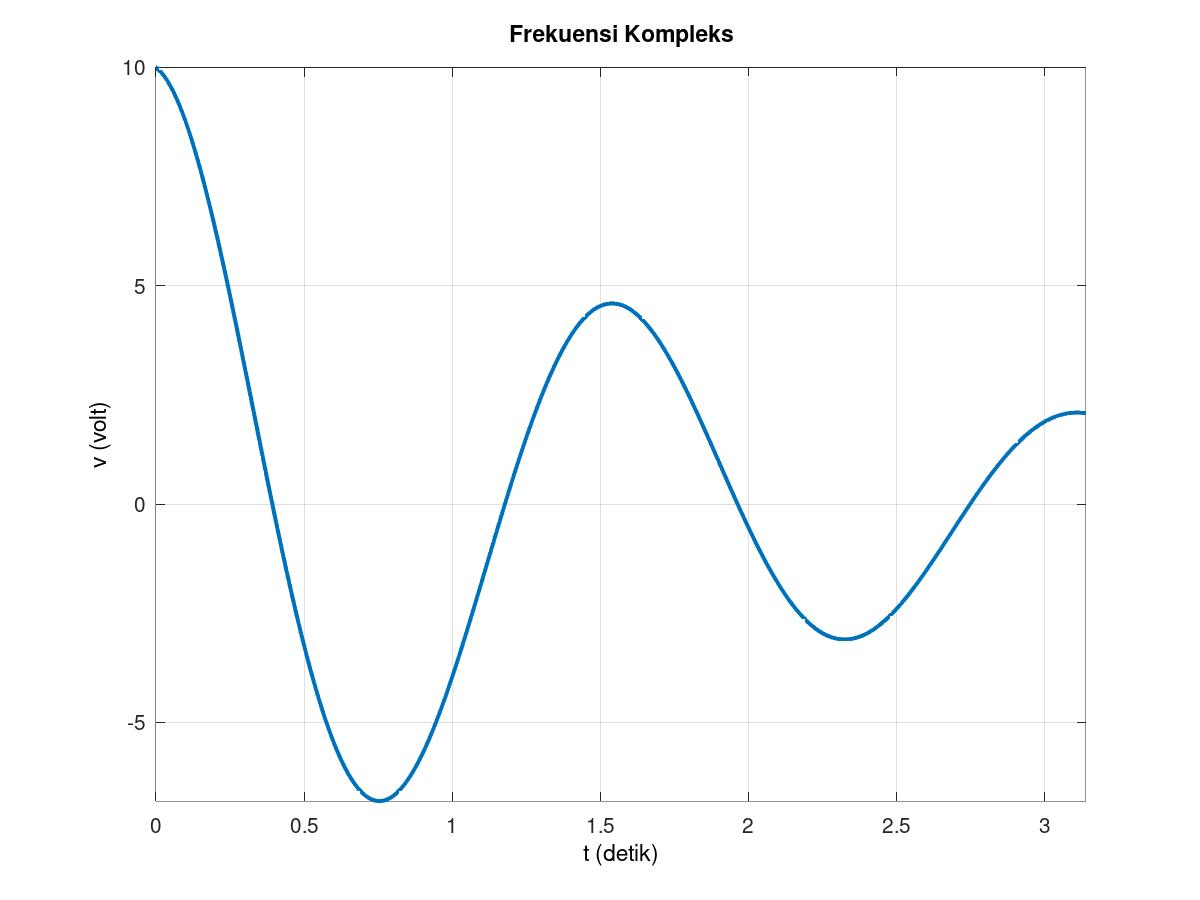
\includegraphics[width=0.8\linewidth]{gambar5.jpg}
    \end{figure}
\end{frame}

\begin{frame}{Frekuensi Kompleks}
    \begin{itemize}
        \item Nilai $\sigma < 0$ maka $v(t) = V_m e^{\sigma t} \cos(\omega t + \theta) $
    \end{itemize}
    \begin{figure}
        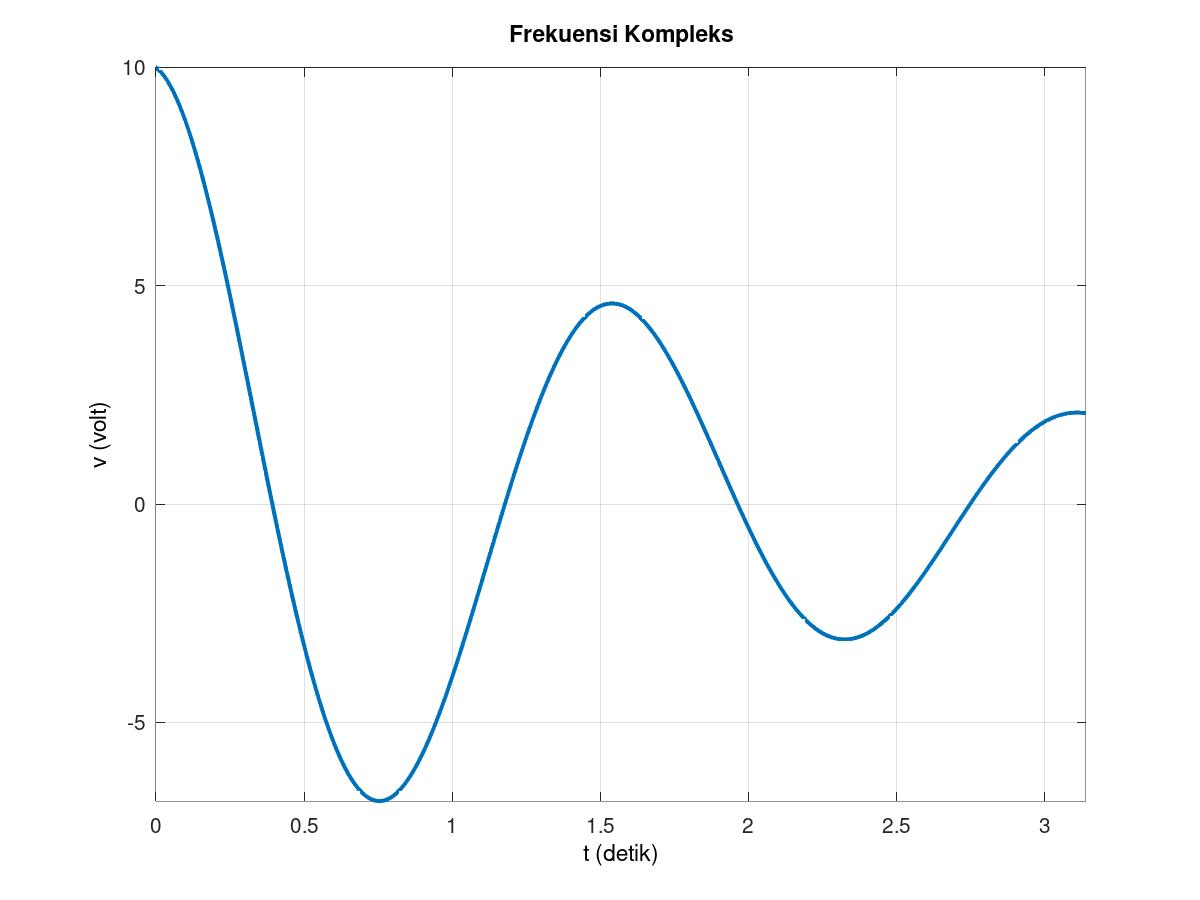
\includegraphics[width=0.8\linewidth]{gambar6.jpg}
    \end{figure}
\end{frame}

\begin{frame}{Frekuensi Kompleks}
    \begin{columns}[T,onlytextwidth]
        \column{0.3\textwidth}
        Fasor sinyal AC
        \begin{align*}
            v(t) &= V_m \cos(\omega t + \theta) \\
            V &= \text{Re} \left[ V_m e^{j(\omega t + \varphi)} \right] \\
            V &= \text{Re} \left[ V_m e^{j(\varphi)} e^{j\omega t} \right] \\
            V(j \omega) &= V_m e^{j \varphi} \\
            V(j\omega) &= V_m \angle \varphi
        \end{align*}

        \column{0.6\textwidth}
        Fasor sinyal frekuensi kompleks
        \begin{align*}
            v(t) &= V_m e^{\sigma t}\cos(\omega t + \theta) \\
            V &= \text{Re} \left[ V_m e^{\sigma t} e^{j(\omega t + \varphi)} \right] \\
            V &= \text{Re} \left[ V_m e^{j(\varphi)} e^{(\sigma + j\omega t)} \right] \leftrightarrow s = \sigma + j \omega\\
            V &= \text{Re} \left[ V_m e^{j \varphi} e^{st}  \right]\\
            V(s) &= V_m e^{j \omega} \\
            V(s) &= V_m \angle \varphi
        \end{align*}
    \end{columns}    
\end{frame}

\begin{frame}
    Impedansi dalam frekuensi kompleks \\~\\
    $$V(s) = \frac{Z(s)}{I(s)}$$
    \begin{columns}[T,onlytextwidth]
        \column{0.5\textwidth}
        \begin{description}
            \item $Z_R(s) = R$
            \item $Z_L(s) = sL$
            \item $Z_C(s) = \frac{1}{sC}$
        \end{description}

        \column{0.5\textwidth}
        \begin{description}
            \item $Y_R(s) = \frac{1}{R}$
            \item $Y_L(s) = \frac{1}{sL}$
            \item $Y_C(s) = sC$
        \end{description}
    \end{columns}
\end{frame}

\begin{frame}{Frekuensi Kompleks}
    \textbf{Contoh Soal} \\
    Tentukan nilai $i(t)$ dari rangkaian berikut ini.
    \begin{columns}
        \column{0.5\textwidth}
            \begin{figure}[]
                \centering
                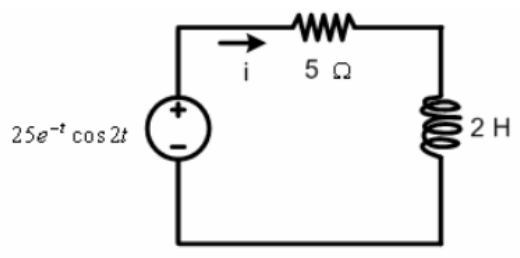
\includegraphics[width=0.8\linewidth]{contoh1.png}
                \caption{}
                \label{}
            \end{figure}

        \column{0.5\textwidth} 
            \begin{align*}
                s       &= \sigma + j \omega \\
                        &= -1 + j2 \\
                Z_R(s)  &= 5 \omega \\
                Z_L(s)  &= sL = 2s \omega \\
                Z_T(s)  &= 5 + 2s \omega \\
                V       &= 25 e^{-t} \cos(2t) = 25 \angle 0^{\circ} \text{v} \\
                i(s)    &= \frac{V(s)}{Z_T(s)} = \frac{25 \angle 0^{\circ}}{5 + 2s} = \frac{25 \angle 0^{\circ}}{5+2(-1)} \\
                        &= 5e^{-t} \cos(2t - 53,1^{\circ}) \text{A}
            \end{align*}
    \end{columns}
\end{frame}

\section{Respon Frekuensi}

\begin{frame}{Respon Frekuensi}
    \begin{itemize}
        \item Jika sebuah sumber sinusoidal dengan amplitudo konstan dan frekuensi yang berubah-ubah, akan didapatkan \alert{respon frekuensi}
    \end{itemize}
\end{frame}
\begin{frame}[standout]
    Ada Pertanyaan?
\end{frame}
  
\appendix
  
\end{document}